\section{Revue élémentaire des méthodes de deep learning}

\subsection{Réseau de neurones}

\begin{frame}{Réseau de neurones}
\begin{figure}[ht!]
\centering
\begin{tabular}{cc}
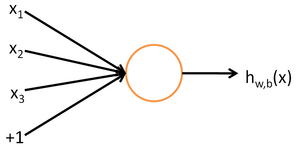
\includegraphics[width = .4\columnwidth]{../fig/SingleNeuron.png} &
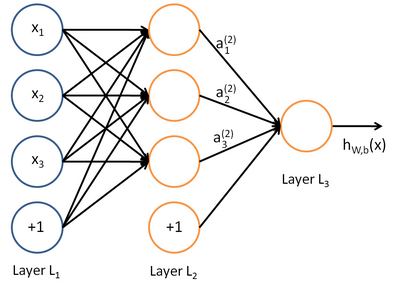
\includegraphics[width = .4\columnwidth]{../fig/Network331.png} 
\end{tabular}
\caption{(gauche) Un neurone avec trois entrées $(x_1,x_2,x_3)$ et un \emph{offset} ; (droite) un réseau de neurones de taille $(3,3,1)$ avec des \emph{offset} aux deux premières couches.}
\label{fig1}
\end{figure}
\begin{block}{Sortie d'un neurone simple}
\begin{equation}
h_{w,b}(x)=\sigma(w^Tx)=\sigma\left(\sum_{i=1}^p w_i x_i + b\right)
\end{equation}
\end{block}
\end{frame}



\subsection{Multilayer Perceptron (MLP)}

\begin{frame}{Multilayer Perceptron (MLP)}
\begin{figure}[ht!]
\centering
\begin{tabular}{cc}
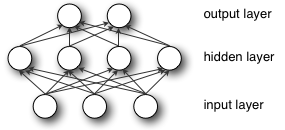
\includegraphics[width = .5\columnwidth]{../fig/mlp} &
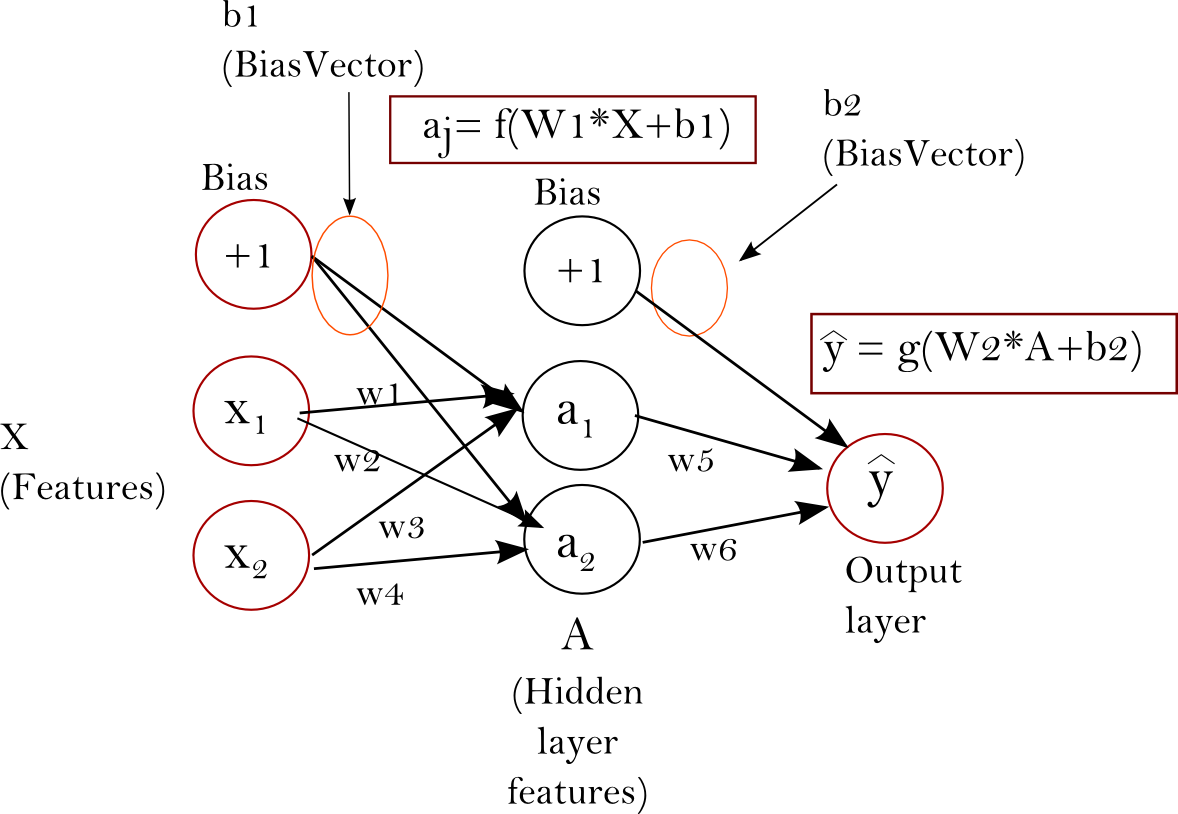
\includegraphics[width = .5\columnwidth]{../fig/backprop_notation.png} 
\end{tabular}
\caption{(gauche) Un MLP avec une seule couche de variables cachées ; (droite) structure de MLP avec l'ajout de biais et les poids.}
\label{fig2}
\end{figure}
\end{frame}



\begin{frame}{Multilayer Perceptron (MLP)}
\begin{block}{Sortie d'un nœud}
\begin{equation}
s(x) = \sigma(Wx + b)
\end{equation}
\end{block}
Le MLP diffère par la manière d'entraîner :
\begin{description}
\item[Forward pass. ]On part des variables visibles $v$ et on remonte le graphe avec les poids de la structure.
\item[Backpropagation. ]Chemin inverse en descendant le graphe et en comptabilisant les erreurs commises, mise à jour les poids.
\end{description}
\end{frame}

